\documentclass[14pt]{beamer}
\usepackage{newtxtext,newtxmath}
\usepackage{microtype}
\usepackage[english]{babel}
\usepackage{hyperref}
\usepackage{graphicx}
\usepackage{listings}
\lstloadlanguages{Python}
\lstset{language=Python}
\lstset{%
basicstyle=\ttfamily\bfseries,
keywordstyle=\color{blue}, emph={self}, emphstyle={\color{blue}},
identifierstyle=,
commentstyle=\color{brown},
stringstyle=\color{green!50!black},
showstringspaces=false,
emphstyle={[2]\color{purple}},
}
\usepackage{tikz}
\usepackage{forest}
\usetikzlibrary{positioning}
\usepackage{array}
\newcolumntype{L}[1]{>{\raggedright\let\newline\\\arraybackslash\hspace{0pt}}m{#1}}

\mode<presentation>{
\usetheme{Madrid}
\definecolor{uabgreen}{cmyk}{.89,.31,.78,.17}
\usecolortheme[named=uabgreen]{structure}
\setbeamertemplate{navigation symbols}{}
\setbeamertemplate{footline}[frame number]
\setbeamertemplate{section in toc}[square]
\setbeamertemplate{subsection in toc}[square]
\setbeamertemplate{items}[square]
\setbeamercovered{transparent=5}
}

\newcommand{\keyword}[1]{{\color{blue}#1}}
\newcommand{\cmnt}[1]{{\color{gray}#1}}
\newcommand{\str}[1]{{\color{green!50!black}#1}}
\newcommand{\defn}[1]{{\color{purple}#1}}

\author[Dr. Bethard]{Dr. Steven Bethard}
\institute[UAB CIS]{%
Computer and Information Sciences\\
University of Alabama at Birmingham}

\AtBeginSection[]
{
  \begin{frame}<beamer>{Outline}
    \tableofcontents[currentsection]
  \end{frame}
}

\tikzset{
  invisible/.style={opacity=0,text opacity=0},
  visible on/.code={%
    \alt<#1>{}{\pgfkeysalso{invisible}}
  },
  filled on/.code={%
    \alt<#1>{\pgfkeysalso{fill=gray}}{}
  },
}
\forestset{
  edge weight/.style={
    edge label={node[midway,above,sloped]{#1}}},
  invisible/.style={
    /tikz/invisible,
    edge={/tikz/invisible}},
  visible on filled on/.code n args={2}{%
    \alt<#1>{\alt<#2>{\pgfkeysalso{fill=gray}}{}}{\pgfkeysalso{invisible}}
  },
  visible on/.code={%
    \alt<#1>{}{\pgfkeysalso{invisible}}
  },
}

\lstset{emph={[2]ReflexVacuumAgent,ReflexWithStateVacuumAgent,take_action,__init__}}

\title{Introduction to Artificial Intelligence}
\date[]{7 Jan 2014}

\begin{document}

\begin{frame}
  \titlepage
\end{frame}

\section*{Introduction}

\subsection*{Who is teaching this course?}
\begin{frame}{Who is teaching this course?}
	\begin{block}{Steven Bethard, Ph.D.}
		\begin{itemize}
			\item Asst. Professor, Computer and Information Sciences
			\item Research:
				\begin{itemize}
					\item Natural language processing
					\item Machine learning
					\item Information retrieval
					\item Clinical and educational applications
				\end{itemize}
		\end{itemize}
	\end{block}
\end{frame}

\subsection*{Who is taking this course?}
\begin{frame}{Who is taking this course?}
	\begin{block}{Index Card Information}
		\begin{enumerate}
			\item Your name
			\item Your major(s) or research area(s)
			\item Why you're interested in Artificial Intelligence
			\item What you expect to learn in this course
			\item How comfortable you are with data structures, \\
			      e.g. hash tables, priority queues, graphs
		\end{enumerate}
	\end{block}
\end{frame}

\subsection*{What will you learn to do in this course?}
\begin{frame}{What will you learn to do in this course?}
	\begin{itemize}
		\item Apply search algorithms to computational problems
		\item Analyze problems using logic and inference
		\item Reason about problems using probabilistic analysis
		\item Train statistical learning methods for classification
	\end{itemize}
\end{frame}

\subsection*{What are the course requirements?}

\begin{frame}{General Information}
	\begin{block}{Times}
		\begin{description}
			\item[Class] Tue, Thu 12:30-13:45
			\item[Office] Tue 13:45-15:00 and by appointment
		\end{description}
	\end{block}
	\begin{block}{Textbook}
		\textit{Artificial Intelligence: A Modern Approach, Third Edition}\\		
		Stuart J. Russell and Peter Norvig\\
		Prentice Hall, 2009.\\
		\hfill \alert{Chessboard cover, not green cover}
	\end{block}
\end{frame}

\begin{frame}{Grading}
\begin{tabular}{@{} r l l @{}}
\hline
 50 & Programming 1: Agents & Java, 2 weeks \\
150 & Programming 2: Search & Java, 2 weeks  \\
150 & Programming 3: Probability & Java, 2 weeks  \\
150 & Programming 4: Learning & Java, 2 weeks  \\
\hline
100 & Quiz 1: Search & In class, 30 minutes \\
100 & Quiz 2: Logic & In class, 30 minutes \\
100 & Quiz 3: Probability & In class, 30 minutes \\
100 & Quiz 4: Learning (Final Exam) & In class, 30 minutes \\
\hline
100 & Class Participation \\
\hline
250 & Class Project (\alert{660/760 only}) & Java, 10 weeks \\
250 & Class Presentation (\alert{760 only}) & In class, 15 minutes \\
\hline
\end{tabular}
\end{frame}

\part{Intelligent Agents}
\begin{frame}{Outline}
  \tableofcontents
\end{frame}

\section{Intelligent Agents}
\subsection{Agents and Environments}

\begin{frame}{Agents and Environments}
	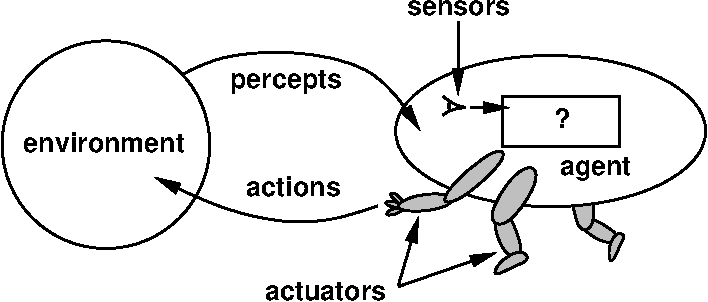
\includegraphics[width=\textwidth]{agent-environment.pdf}
\end{frame}

\subsection{Example: Vacuum Cleaner World}

\begin{frame}{Vacuum Cleaner World}
	\begin{center}
		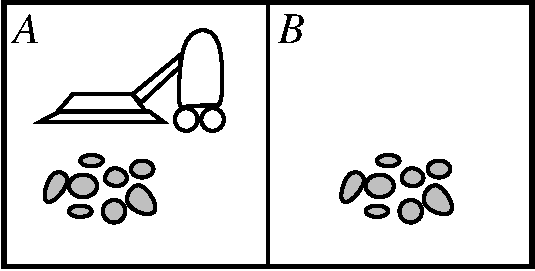
\includegraphics[width=3in]{vacuum-environment.pdf}
	\end{center}
	\begin{description}
		\item[Percepts:] Location and status, e.g. [\textit{A, Dirty}]
		\item[Actions:] \textit{Left, Right, Suck, NoOp}
	\end{description}
\end{frame}

\begin{frame}[fragile]{A Vacuum Cleaner Agent}
	\begin{lstlisting}
		class ReflexVacuumAgent(object):
			    def take_action(self, percept):
		        location, status = percept
		        if status == "Dirty":
		            return "Suck"
		        elif location == "A":
		            return "Right"
		        elif location == "B":
		            return "Left"
	\end{lstlisting}
\end{frame}

\subsection{Rational Agents}

\begin{frame}{Rational Agents}
	\begin{block}{Performance Measure}
		How successful was the agent?
		
		\textit{
		E.g. the vacuum cleaner agent:
		\begin{itemize}[<2->]
			\item Maximized clean squares
			\item Minimized electricity consumed
		\end{itemize}
		}
	\end{block}	
	\uncover<3->{
	\begin{block}{Rational Agent}
		Selects the action that is expected to maximize the performance measure
	\end{block}
	}
\end{frame}

\begin{frame}{Rational vs. Omniscient}
	\begin{block}{Rational?}
		\begin{itemize}
			\item Left turn arrow was red. Didn't check for oncoming traffic. Turned left. Hit by a bus.
			\pause
			\item Left turn arrow was green. Didn't check for oncoming traffic. Turned left. Hit by a bus.
			\pause
			\item Left turn arrow was green. Checked for oncoming traffic, saw none. Turned left. Hit by bus.
		\end{itemize}
	\end{block}	
\end{frame}

\section{Environment Types}

\subsection{Specifying the Task}

\begin{frame}{Specifying a Driving Task}
	\begin{block}{Performance measure}
		\uncover<2->{safety, destination, profts, legality, comfort\ldots}
	\end{block}
	\begin{block}{Environment}
		\uncover<3->{streets/freeways, traffic, pedestrians, weather\ldots}
	\end{block}
	\begin{block}{Actuators}
		\uncover<4->{steering, accelerator, brake, speaker/display\ldots}
	\end{block}
	\begin{block}{Sensors}
		\uncover<5->{video, accelerometer, microphone, GPS\ldots}
	\end{block}
\end{frame}

\subsection{Describing Environments}

\begin{frame}{Describing Environments}
	\begin{block}{Fully vs. Partially Observable}
		\begin{description}
			\item[Fully] All relevant to action is visible, e.g. \textit{chess}
			\item[Partially] Part of environment unavailable, e.g. \textit{poker}
		\end{description}
	\end{block}
	\begin{block}{Deterministic vs. Strategic vs. Stochastic}
		\begin{description}
			\item[Determin.] State + action determines next state, \\ e.g. \textit{crossword}
			\item[Strategic] State + action + other agent actions determines next state, e.g. \textit{chess}
			\item[Stochastic] Next state not fully determined, e.g. \textit{poker}
		\end{description}
	\end{block}
\end{frame}
\begin{frame}{Describing Environments}
	\begin{block}{Episodic vs. Sequential}
		\begin{description}
			\item[Episodic] Old actions irrelevant, e.g. \textit{face detection}
			\item[Sequential] Old actions affect current state, e.g. \textit{chess}
		\end{description}
	\end{block}
	\begin{block}{Static vs. Semidynamic vs. Dynamic}
		\begin{description}
			\item[Static] Environment does not change while deciding, e.g. \textit{chess, poker}
			\item[Semi] Performance score changes while deciding, e.g. \textit{face detection}
			\item[Dynamic] Environment changes while deciding, \\ e.g. \textit{driving}
		\end{description}
	\end{block}
\end{frame}
\begin{frame}{Describing Environments}
	\begin{block}{Discrete vs. Continuous}
		\begin{description}
			\item[Discrete] States, percepts and actions are countable, e.g. \textit{chess, poker}
			\item[Continuous] States, percepts or actions are real-valued, e.g. \textit{driving}
		\end{description}
	\end{block}
	\begin{block}{Single vs. Multiple Agents}
		\begin{description}
			\item[Single] Single agent, e.g. \textit{crossword, face detection}
			\item[Multiple] More than one agent, e.g. \textit{poker, driving}
		\end{description}
	\end{block}
\end{frame}

\subsection{Example Environments}

\newcommand{\U}[2]{\uncover<#1->{#2}}
\begin{frame}{Example Environments}

	{\small
	\begin{tabular}{lcccc}
		              &                  &                  & Internet        &      \\
		              & Solitaire        & Chess            & Shopping        & Taxi \\
		\hline
		Observable    & \U{2}{No}        & \U{2}{Yes}       & \U{2}{No}       & \U{2}{No}\\
		Deterministic & \U{3}{No}        & \U{3}{Strategic} & \U{3}{Partly}   & \U{3}{No}\\
		Episodic      & \U{4}{No}        & \U{4}{No}        & \U{4}{No}       & \U{4}{No}\\
		Static        & \U{5}{Yes}       & \U{5}{Yes}       & \U{5}{Semi}     & \U{5}{No}\\
		Discrete      & \U{6}{Yes}       & \U{6}{Yes}       & \U{6}{Yes}      & \U{6}{No}\\
		Single-agent  & \U{7}{Yes}       & \U{7}{No}        & \U{7}{Maybe}    & \U{7}{No}\\
	\end{tabular}
	}
\end{frame}

\section{Agent Types}

\subsection{Reflex Agents}

\begin{frame}{Simple Reflex Agents}
	\begin{center}
		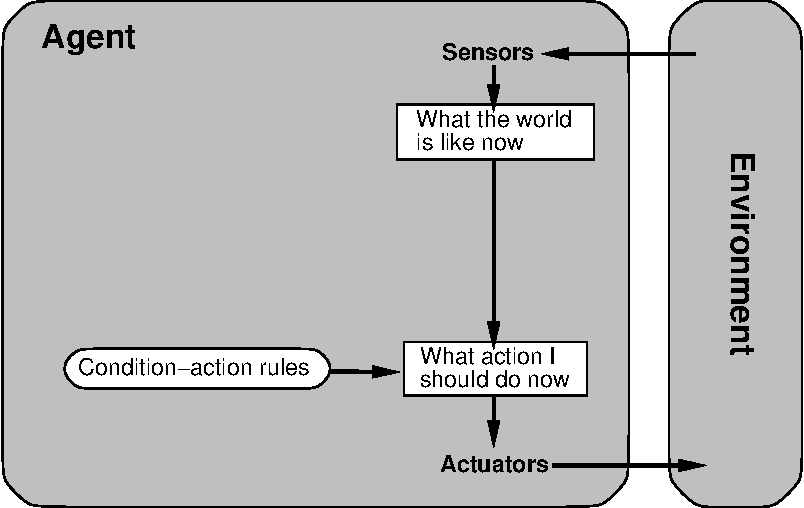
\includegraphics[width=3in]{simple-reflex-agent.pdf}
	\end{center}
\end{frame}

\begin{frame}[fragile]{Simple Reflex Agent Example}
	\begin{lstlisting}
		class ReflexVacuumAgent(object):
		    def take_action(self, percept):
		        location, status = percept
		        if status == "Dirty":
		            return "Suck"
		        elif location == "A":
		            return "Right"
		        elif location == "B":
		            return "Left"
	\end{lstlisting}
\end{frame}

\begin{frame}{Stateful Reflex Agents}
	\begin{center}
		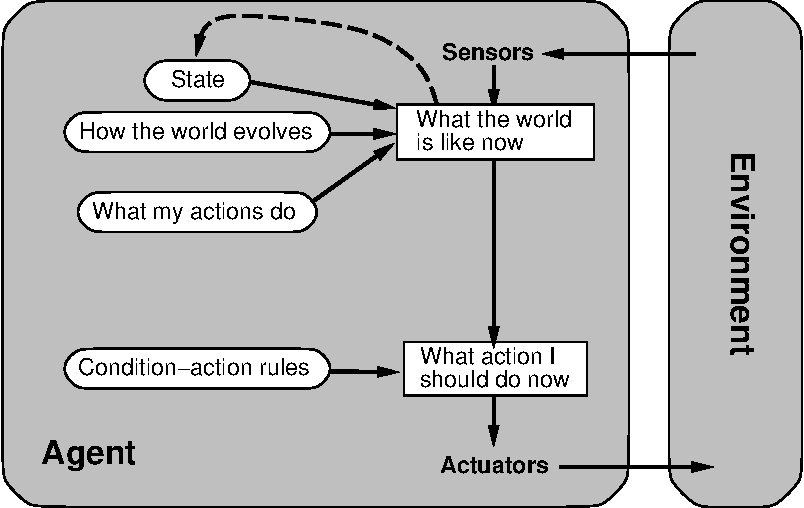
\includegraphics[width=3in]{reflex+state-agent.pdf}
	\end{center}
\end{frame}

\begin{frame}[fragile]{Stateful Reflex Agent Example}
	\footnotesize
	\begin{lstlisting}
		class StatefulReflexVacuumAgent(object):
		    def __init__(self):
		        self.time_at_location = 3
		        self.directions = dict(A="Right", B="Left")
		    def take_action(self, percept):
		        self.time_at_location += 1
		        location, status = percept
		        if status == "Dirty":
		            return "Suck"
		        elif self.time_at_location > 3:
		            self.time_at_location = 0
		            return self.directions[location]
		        else:
		            return "NoOp"
	\end{lstlisting}
\end{frame}


\subsection{Goal-based Agents}
\begin{frame}{Goal-based Agents}
	\begin{center}
		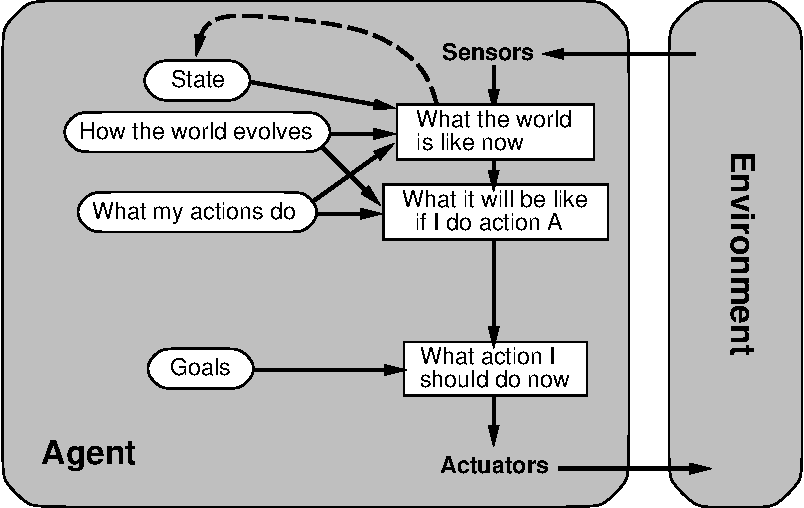
\includegraphics[width=3in]{goal-based-agent.pdf}
	\end{center}
\end{frame}

\subsection{Utility-based Agents}
\begin{frame}{Utility-based Agents}
	\begin{center}
		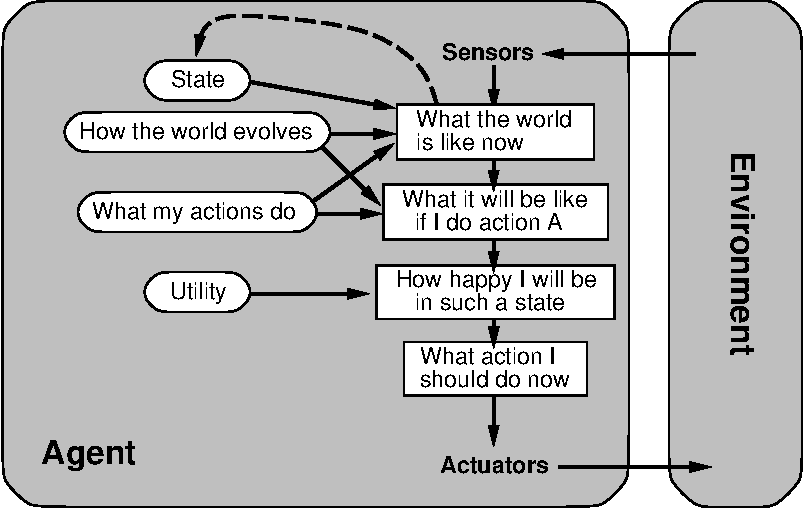
\includegraphics[width=3in]{utility-based-agent.pdf}
	\end{center}
\end{frame}

\subsection{Learning Agents}
\begin{frame}{Learning Agents}
	\begin{center}
		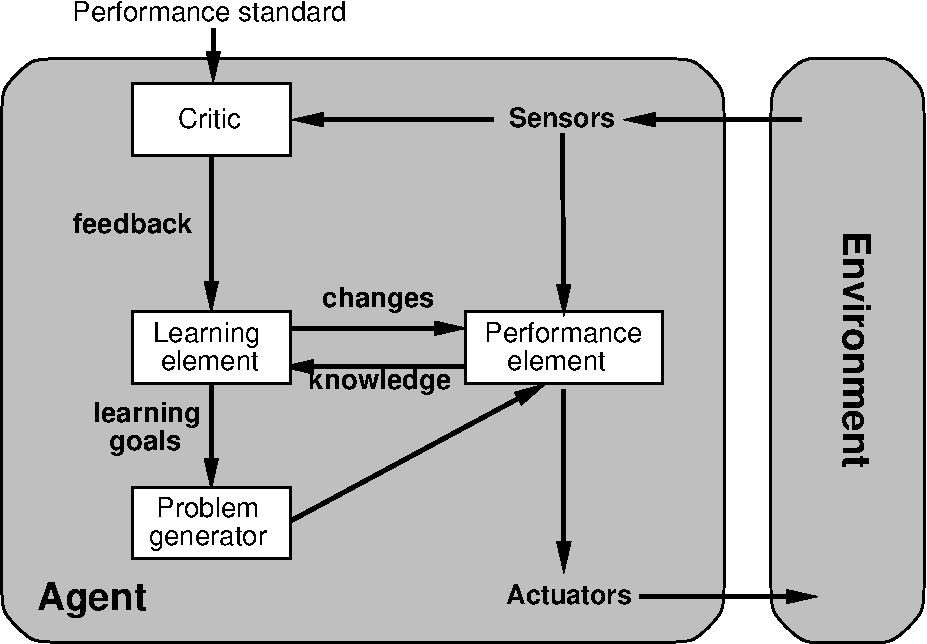
\includegraphics[width=3in]{learning-agent.pdf}
	\end{center}
\end{frame}

\section*{Key Points}
\begin{frame}{Key Points}
	\begin{itemize}
		\item Agents take \alert<2->{actions} based on \alert<2->{percepts}
		\item Rational agents maximize a \alert<3->{performance measure}
		\item Features of task environments:
			\begin{itemize}
				\item
					\alert<4->{Observable}?
					\alert<4->{Deterministic}?
					\alert<4->{Episodic}? \\
					\alert<4->{Static}?
					\alert<4->{Discrete}?
					\alert<4->{Single-agent}?
			\end{itemize}
		\item Agent architectures:
			\begin{itemize}
				\item
					\alert<5->{Reflex},
					\alert<5->{Stateful reflex},
					\alert<5->{Goal-based},
					\alert<5->{Utility-based}
			\end{itemize}
	\end{itemize}
\end{frame}

\end{document}
